\documentclass[11pt]{article}

\usepackage[margin=1in]{geometry}
\usepackage{amsmath,amssymb}
\usepackage{booktabs}
\usepackage{graphicx}
\usepackage{hyperref}
\usepackage{xcolor}
\usepackage{caption}
\usepackage{float}
\usepackage{natbib}

\hypersetup{
    colorlinks=true,
    linkcolor=blue,
    citecolor=blue,
    urlcolor=blue
}

\title{C-CATM: Cross-Turn Contrastive Activation Trajectory Monitor \\ for Multi-Turn LLM Jailbreak Detection}

\author{Neerav Gupta \\ \normalsize Independent Research}

\date{}

\begin{document}

\maketitle

\begin{center}
\textbf{Code:} \url{https://github.com/Neerav-Gupta/C-CATM} \\
\textbf{Models:} \url{https://huggingface.co/Neerav-Gupta/ccatm-safety-monitor}
\end{center}

\begin{abstract}
Multi-turn jailbreak attacks---including crescendo escalation, contextual reframing, and iterative goal decomposition---routinely bypass single-turn safety classifiers by distributing harmful intent across a conversation rather than concentrating it in one message. We introduce \textbf{C-CATM} (Cross-turn Contrastive Activation Trajectory Monitor), a lightweight safety monitor that operates directly on a target model's hidden-state trajectory across turns rather than on its output text. C-CATM combines (1) a learned trajectory encoder trained with a supervised contrastive objective on turn-to-turn activation deltas, and (2) a constitutional gating layer that maps trajectory embeddings to a calibrated safety probability. We evaluate C-CATM against three baseline monitors (Llama Guard, an activation-drift monitor we call TrajGuard, and a rule-based Constitutional monitor) across two target models (Llama-3.1-8B-Instruct and Qwen2.5-7B-Instruct) and four multi-turn attack strategies (Crescendo, Jigsaw, Echo Chamber, Safe-in-Isolation), totaling 1{,}192 evaluated conversation traces. C-CATM achieves a substantially lower false-positive rate than all baselines on Llama-3.1-8B (2.3\% vs.\ 6.1--88.3\%) while maintaining competitive recall (50.0\%), and generalizes to an unseen model architecture (Qwen2.5-7B) with an F1 of 61.1, exceeding all baselines on that model as well. An ablation study shows the learned trajectory encoder is responsible for the bulk of this performance (+22.0 F1 points over a randomly initialized encoder of identical architecture), while the constitutional rule-scoring component, in its current trained form, contributes negligibly to the final decision---a finding we report transparently as it bears on how the architecture should be interpreted and improved. C-CATM's monitor-only inference latency is 6.2ms per trace. We release all code, trained weights, and evaluation harness for reproducibility.
\end{abstract}

\section{Introduction}

Large language models deployed in production are commonly protected by safety classifiers that inspect a single input-output pair for policy violations. This works reasonably well against single-turn attacks but is known to be far less effective against \textbf{multi-turn jailbreaks}, where an attacker spreads harmful intent across several conversational turns---gradually escalating a request (Crescendo) \citep{russinovich2024crescendo}, splitting a harmful task into individually-innocuous sub-requests (Jigsaw) \citep{yang2024jigsaw}, building shared fictional or academic context that reframes a later request as acceptable (Echo Chamber) \citep{alobaid2026echochamber}, or requesting a component of a harmful task ``in isolation'' so that no single turn looks harmful (Safe-in-Isolation) \citep{srivastav2025safeinisolation}. Large-scale human red-teaming studies confirm that these strategies are not isolated curiosities: manually constructed multi-turn conversations bypass current defenses at far higher rates than single-turn attacks across a wide range of deployed models \citep{li2024mhj}.

A natural response is to look not just at any single turn's output, but at how the model's internal state \emph{evolves} across the conversation. Prior work in activation-based monitoring has shown that a model's hidden states shift measurably along safety-relevant directions as it is walked toward unsafe generation. However, naively thresholding activation drift (which we implement here as a baseline, ``TrajGuard'') produces extremely high false-positive rates, because normal topic shifts and stylistic variation also move activations substantially.

We propose C-CATM, which instead of using a single linear ``safety direction,'' \textbf{learns} a trajectory encoder via a supervised contrastive objective to distinguish the \emph{shape} of safe vs.\ unsafe conversational trajectories, and combines this with a constitutional rule-scoring layer intended to add interpretability and cross-model transfer.

\paragraph{Contributions.}
\begin{enumerate}
    \item A trajectory-based safety monitor (C-CATM) that operates on turn-to-turn hidden-state deltas, achieving substantially lower false-positive rates than text-based and naive activation-based baselines at comparable recall.
    \item A cross-model evaluation showing the approach transfers from Llama-3.1-8B to the architecturally distinct Qwen2.5-7B without retraining.
    \item An honest ablation study, including a negative result: the constitutional rule-scoring component, as currently trained, does not measurably influence the monitor's decisions, and we discuss why.
    \item A fully reproducible, open-source evaluation harness (four attacks $\times$ five monitors $\times$ two target models), trained model weights, and all evaluation data.
\end{enumerate}

\section{Related Work}

\paragraph{Single-turn safety classifiers.} Guard models such as Llama Guard \citep{inan2023llamaguard}, ShieldGemma \citep{zeng2024shieldgemma}, WildGuard \citep{han2024wildguard}, and OpenAI's production moderation classifier \citep{markov2023moderation} classify a single prompt-response pair against a fixed taxonomy of harm categories. These are effective against direct harmful requests but are not designed to reason about intent distributed across a conversation; we use Llama Guard as our representative text-based baseline (Section~4) because it is the most widely adopted open-weight guard model in the multi-turn jailbreak literature we build on below.

\paragraph{Single-turn adversarial jailbreaks.} Before multi-turn strategies, a substantial line of work focused on constructing single adversarial prompts that induce harmful completions in one shot: gradient-based suffix optimization \citep{zou2023gcg}, iterative black-box refinement using an attacker LLM \citep{chao2023pair}, and tree-structured search over candidate prompts \citep{mehrotra2023tap}. These methods established that a single, sufficiently optimized turn can bypass alignment; multi-turn strategies extend this observation by showing that even \emph{unoptimized}, individually-benign-looking turns can achieve similar effects when the harmful intent is spread across a conversation.

\paragraph{Multi-turn jailbreaks.} A growing body of red-teaming literature documents attacks that succeed specifically by exploiting multi-turn context: gradual escalation strategies such as Crescendo \citep{russinovich2024crescendo}, decomposition of a harmful task into benign-looking sub-questions (Jigsaw) \citep{yang2024jigsaw}, agent-driven decomposition of a harmful task into individually-safe-looking sub-components (Safe-in-Isolation) \citep{srivastav2025safeinisolation}, and the use of shared fictional or conversational framing to normalize a later harmful request (Echo Chamber) \citep{alobaid2026echochamber}. Beyond these four strategies, recent work has documented a broader and still-growing space of multi-turn attack constructions and defenses, including semantic-driven contextual attack chains \citep{yang2024chainofattack}, first-principles analyses of what makes multi-turn context exploitable \citep{sun2024multiturncontext}, adaptive multi-agent attacker/defender frameworks \citep{rahman2024xteaming}, and state-dependent safety failures that emerge only after specific conversational states are reached \citep{li2026star}, alongside the large-scale human-jailbreak study noted above \citep{li2024mhj}. These attacks are the motivating threat model for this work. Our implementations of Jigsaw, Echo Chamber, and Safe-in-Isolation are our own, built to match the high-level strategy described in the respective papers above rather than using the original authors' released code, exact prompts, or agent scaffolding (see Section~\ref{sec:limitations}).

\paragraph{Activation-based monitoring and steering.} Separately, work on activation steering and linear probing has shown that many safety-relevant behaviors correspond to reasonably linear directions in a model's residual stream: refusal behavior in particular has been shown to be mediated by a single, extractable direction \citep{arditi2024refusal}, and contrastive activation addition has been used to steer generation along similar directions at inference time \citep{rimsky2023caa}. Representation engineering has been proposed more broadly as a top-down framework for reading and controlling model-internal state \citep{zou2023repe}, and related probing work has found that other latent properties---not just safety or refusal---admit similarly linear structure, whether recovered via unsupervised consistency objectives \citep{burns2022latentknowledge} or found to emerge directly from simple true/false statement representations \citep{marks2023geometryoftruth}. Circuit-breaker approaches take this further by training representation-level interventions directly into the model to short-circuit harmful generation \citep{zou2024circuitbreakers}. This body of work motivates using hidden states, rather than only text, as a monitor's input signal. Our TrajGuard baseline is a direct, simplified implementation of the single-direction idea (a fitted linear safety direction), which we find performs poorly as a \emph{standalone} multi-turn monitor due to high variance in what counts as ``safety-relevant'' drift across ordinary conversations---suggesting that a single static direction, however well it works for steering or refusal-detection in single-turn settings, is insufficient to characterize a multi-turn \emph{trajectory}.

\paragraph{Interpretable feature extraction.} Sparse autoencoders have been used to recover human-interpretable features from language model activations \citep{cunningham2023sae}. We explored an SAE-based approach for extracting our constitutional concept vectors (Section~3.2) before ultimately using a simpler linear-probe extraction for training stability and speed; we discuss this choice in Section~\ref{sec:limitations}.

\paragraph{Constitutional AI.} Constitutional approaches use a fixed set of natural-language rules or principles to guide or evaluate model behavior \citep{bai2022constitutional}. We incorporate a constitutional rule-scoring layer into C-CATM's gate, both for interpretability and as a hand-designed inductive bias, and report an ablation examining whether this component is actually used by the trained model.

\paragraph{Evaluation resources.} We use HarmBench \citep{mazeika2024harmbench} as our source of harmful behaviors and as our ground-truth harmfulness classifier, and a StrongReject-style \citep{souly2024strongreject} continuous score for auxiliary analysis. JailbreakBench \citep{chao2024jailbreakbench} provides a similar standardized behavior set and evaluation protocol for jailbreak robustness research and is a natural target for extending this evaluation beyond HarmBench in future work.

\section{Method}

\subsection{Threat Model and Evaluation Harness}

We built a multi-turn red-teaming harness consisting of:

\begin{itemize}
    \item \textbf{Four attackers:} Crescendo (gradual escalation across up to 10 turns, using the target model itself as its own attacker LLM), Jigsaw (decomposition of a harmful behavior into sub-tasks across up to 6 turns), Echo Chamber (context-building across up to 8 turns), and Safe-in-Isolation (requesting harmful sub-components framed as individually benign, up to 5 turns).
    \item \textbf{Five monitors:} No Defense (control), Llama Guard (Llama-Guard-3-8B), TrajGuard (a fitted linear activation-drift probe), Constitutional (a rule-based monitor built on Llama Guard plus a fixed constitution), and C-CATM (this work).
    \item \textbf{Two scorers:} a HarmBench classifier (\texttt{cais/HarmBench-Llama-2-13b-cls}) producing a binary harmful/not-harmful label (HB) used as ground truth for our evaluation metrics, and a StrongReject-style continuous score (SR) used for auxiliary analysis.
    \item \textbf{Behaviors:} a stratified subset of HarmBench behaviors across harm categories (200 behaviors for the primary target model, 98 for the secondary target model; 14 behaviors requiring reproduction of copyrighted song lyrics were excluded from the corpus used with secondary models to avoid generation-time content issues unrelated to the safety question under study).
\end{itemize}

Each \emph{cell} in our evaluation matrix corresponds to one (behavior, attack, monitor) triple: the attacker runs its full multi-turn conversation against the target model, the monitor is run against the resulting trajectory, and HarmBench scores the final response for ground-truth harmfulness.

\subsection{C-CATM Architecture}

C-CATM consists of two trained components operating on a target model's residual-stream hidden states, extracted from a fixed layer during each assistant turn.

\paragraph{Trajectory Encoder.} For a conversation of $T$ turns, we extract the target model's hidden state at each turn, truncate or zero-pad it to a common dimension ($d=3584$, the smallest hidden dimension among evaluated target models, to avoid interpolation artifacts), and $L_2$-normalize each turn's vector. Rather than encoding the raw (normalized) hidden states directly, C-CATM encodes the \textbf{sequence of turn-to-turn deltas}: the first turn is represented by its raw normalized activation, and every subsequent turn is represented by the (re-normalized) difference between its activation and the previous turn's activation. This delta representation is designed to capture the \emph{direction of change} in the model's internal state as the conversation progresses, rather than its absolute position in activation space---motivated by the observation that raw hidden states across unrelated conversations are highly cosine-similar (mean pairwise similarity $\approx 0.67$ in our data), while turn-to-turn deltas from safe vs.\ unsafe trajectories are nearly orthogonal (mean cosine similarity $\approx -0.005$, vs.\ $\approx 0.89$ for safe-safe pairs). A small transformer with a learned CLS token processes this delta sequence and outputs a 256-dimensional trajectory embedding.

The encoder is trained with a supervised contrastive loss \citep{khosla2020supcon} on labeled safe/unsafe trajectories, using a class-balanced batch sampler that guarantees a minimum number of unsafe examples per batch (given substantial class imbalance in the training data: 92 unsafe vs.\ 1{,}675 safe trajectories). We found the naive vectorized log-sum-exp formulation of this loss numerically unstable at the similarity ranges produced by normalized delta embeddings, and replaced it with an explicit per-positive-pair computation. The encoder reaches a best contrastive separation ratio of 0.87 between safe and unsafe trajectory clusters---below an a priori target of 2.0---which we attribute to the limited number and diversity of unsafe training trajectories (spanning three model architectures and four attack types) rather than to an architectural failure; we discuss this limitation in Section~\ref{sec:limitations}.

\paragraph{Constitutional Gate.} A fixed constitution of 32 natural-language safety rules is encoded into concept vectors via a linear probe over a mid-network layer (layer 20) of Llama-3.1-8B-Instruct, trained to separate rule-relevant from rule-irrelevant activations (100\% training accuracy).\footnote{Our codebase also supports extracting concept vectors via a pretrained sparse autoencoder release \citep{cunningham2023sae}; we used the linear-probe method for the results in this paper after finding it faster to train and more numerically stable than the SAE-based pipeline in our setting. We did not perform a systematic comparison between the two extraction methods and flag this as an open question rather than a settled result.} The gate combines the trajectory embedding with these concept-similarity scores through a small bridge network and a learned combiner, trained via class-weighted binary cross-entropy (positive class weighted $\approx 18.2\times$ to offset the safe/unsafe imbalance) to output a final calibrated safety probability. This gate reaches 97.1\% training-set accuracy, 68.8\% precision, and 83.7\% recall at a 0.5 decision threshold on the training split before subsequent threshold optimization (Section~\ref{sec:threshold}).

\subsection{Training Data}

Trajectory training data was assembled from hidden-state traces collected during our own evaluation runs across three target models (Llama-3.1-8B, Qwen2.5-7B, and Gemma-3-12B; see Section~\ref{sec:setup} for why Gemma was later excluded from the main evaluation), yielding 1{,}767 training trajectories (92 unsafe) and 317 held-out validation trajectories (20 unsafe) after filtering.

\section{Experimental Setup}
\label{sec:setup}

\paragraph{Target models.} Meta-Llama-3.1-8B-Instruct (primary) and Qwen2.5-7B-Instruct (secondary), evaluated on 200 and 98 stratified HarmBench behaviors respectively, each against all four attacks. We also attempted evaluation on Gemma-3-12B-it but excluded it from the final results due to a large disparity in per-cell inference latency on our available hardware, which made completing the full evaluation matrix impractical within our compute budget; we did not have complete Gemma results at the time of writing and do not report partial results to avoid an unfair comparison based on an incomplete behavior sample.

\paragraph{Compute.} All evaluations were run on a single NVIDIA A100-SXM4-80GB or L40-48GB GPU. C-CATM training (contrastive encoder + gate) took under an hour total on an L40.

\paragraph{Metrics.} For each (target model, monitor) pair we report False Positive Rate (FPR, the fraction of \emph{not-harmful} HarmBench-labeled responses the monitor incorrectly flags), Precision (fraction of flagged responses that are truly harmful), Recall (fraction of truly harmful responses the monitor flags), and F1 (harmonic mean of Precision and Recall).

\paragraph{Baselines.}
\begin{itemize}
    \item \emph{No Defense}: a control that never flags anything (FPR=0\%, Recall=0\% by construction).
    \item \emph{Llama Guard}: Llama-Guard-3-8B \citep{inan2023llamaguard} applied to the final assistant turn.
    \item \emph{TrajGuard}: a linear safety direction fitted from the difference in mean hidden-state activations between 10 held-out safe prompts and 10 held-out harmful behavior prompts (calibrated per target model), thresholded at the midpoint between the mean safe and mean unsafe projection scores.
    \item \emph{Constitutional}: a monitor built on Llama Guard combined with the fixed 32-rule constitution described above.
\end{itemize}

\section{Results}

\subsection{Main Comparison}

\begin{table}[H]
\centering
\caption{Llama-3.1-8B-Instruct (200 behaviors $\times$ 4 attacks; C-CATM evaluated on all 800 resulting cells, other monitors on 1{,}600 cells reflecting an earlier, larger monitor sweep over the same attack traces).}
\label{tab:llama}
\begin{tabular}{lccccccc}
\toprule
Monitor & FPR & Precision & Recall & F1 & TP & FP & FN \\
\midrule
No Defense & 0.0\% &---& 0.0\% & 0.0 & 0 & 0 & 36 \\
Llama Guard & 8.5\% & 13.6\% & 58.3\% & 22.1 & 21 & 133 & 15 \\
TrajGuard & 88.3\% & 2.3\% & 88.9\% & 4.4 & 32 & 1381 & 4 \\
Constitutional & 6.1\% & 15.0\% & 47.2\% & 22.8 & 17 & 96 & 19 \\
\textbf{C-CATM} & \textbf{2.3\%} & \textbf{43.8\%} & \textbf{50.0\%} & \textbf{46.7} & 14 & 18 & 14 \\
\bottomrule
\end{tabular}
\end{table}

\begin{table}[H]
\centering
\caption{Qwen2.5-7B-Instruct (98 stratified behaviors $\times$ 4 attacks).}
\label{tab:qwen}
\begin{tabular}{lccccccc}
\toprule
Monitor & FPR & Precision & Recall & F1 & TP & FP & FN \\
\midrule
No Defense & 0.0\% &---& 0.0\% & 0.0 & 0 & 0 & 124 \\
Llama Guard & 47.3\% & 23.8\% & 77.4\% & 36.4 & 96 & 308 & 28 \\
TrajGuard & 100.0\% & 16.0\% & 100.0\% & 27.6 & 124 & 651 & 0 \\
Constitutional & 47.3\% & 23.8\% & 77.4\% & 36.4 & 96 & 308 & 28 \\
\textbf{C-CATM} & \textbf{19.1\%} & \textbf{46.6\%} & \textbf{88.7\%} & \textbf{61.1} & 55 & 63 & 7 \\
\bottomrule
\end{tabular}
\end{table}

C-CATM achieves the best F1 on both target models, and the lowest FPR among monitors with non-trivial recall on both models. Notably, all baselines degrade sharply on Qwen relative to Llama (e.g., Llama Guard's FPR rises from 8.5\% to 47.3\%), while C-CATM's FPR rises more moderately (2.3\% $\to$ 19.1\%). We note that Qwen is substantially less aligned against our attack suite in absolute terms (124 harmful responses out of 392 cells vs.\ 36 out of 1{,}600 on the larger Llama sweep), so part of this cross-model gap likely reflects task difficulty rather than a pure generalization failure; we discuss this caveat further in Section~\ref{sec:limitations}.

We also observe that the Constitutional monitor produces numerically identical results to Llama Guard on Qwen. This is expected given our Constitutional monitor's implementation wraps Llama Guard's classification and augments it with the fixed constitution; on Qwen, its behavior did not diverge from the underlying Llama Guard classification in our sample.

\begin{figure}[H]
\centering
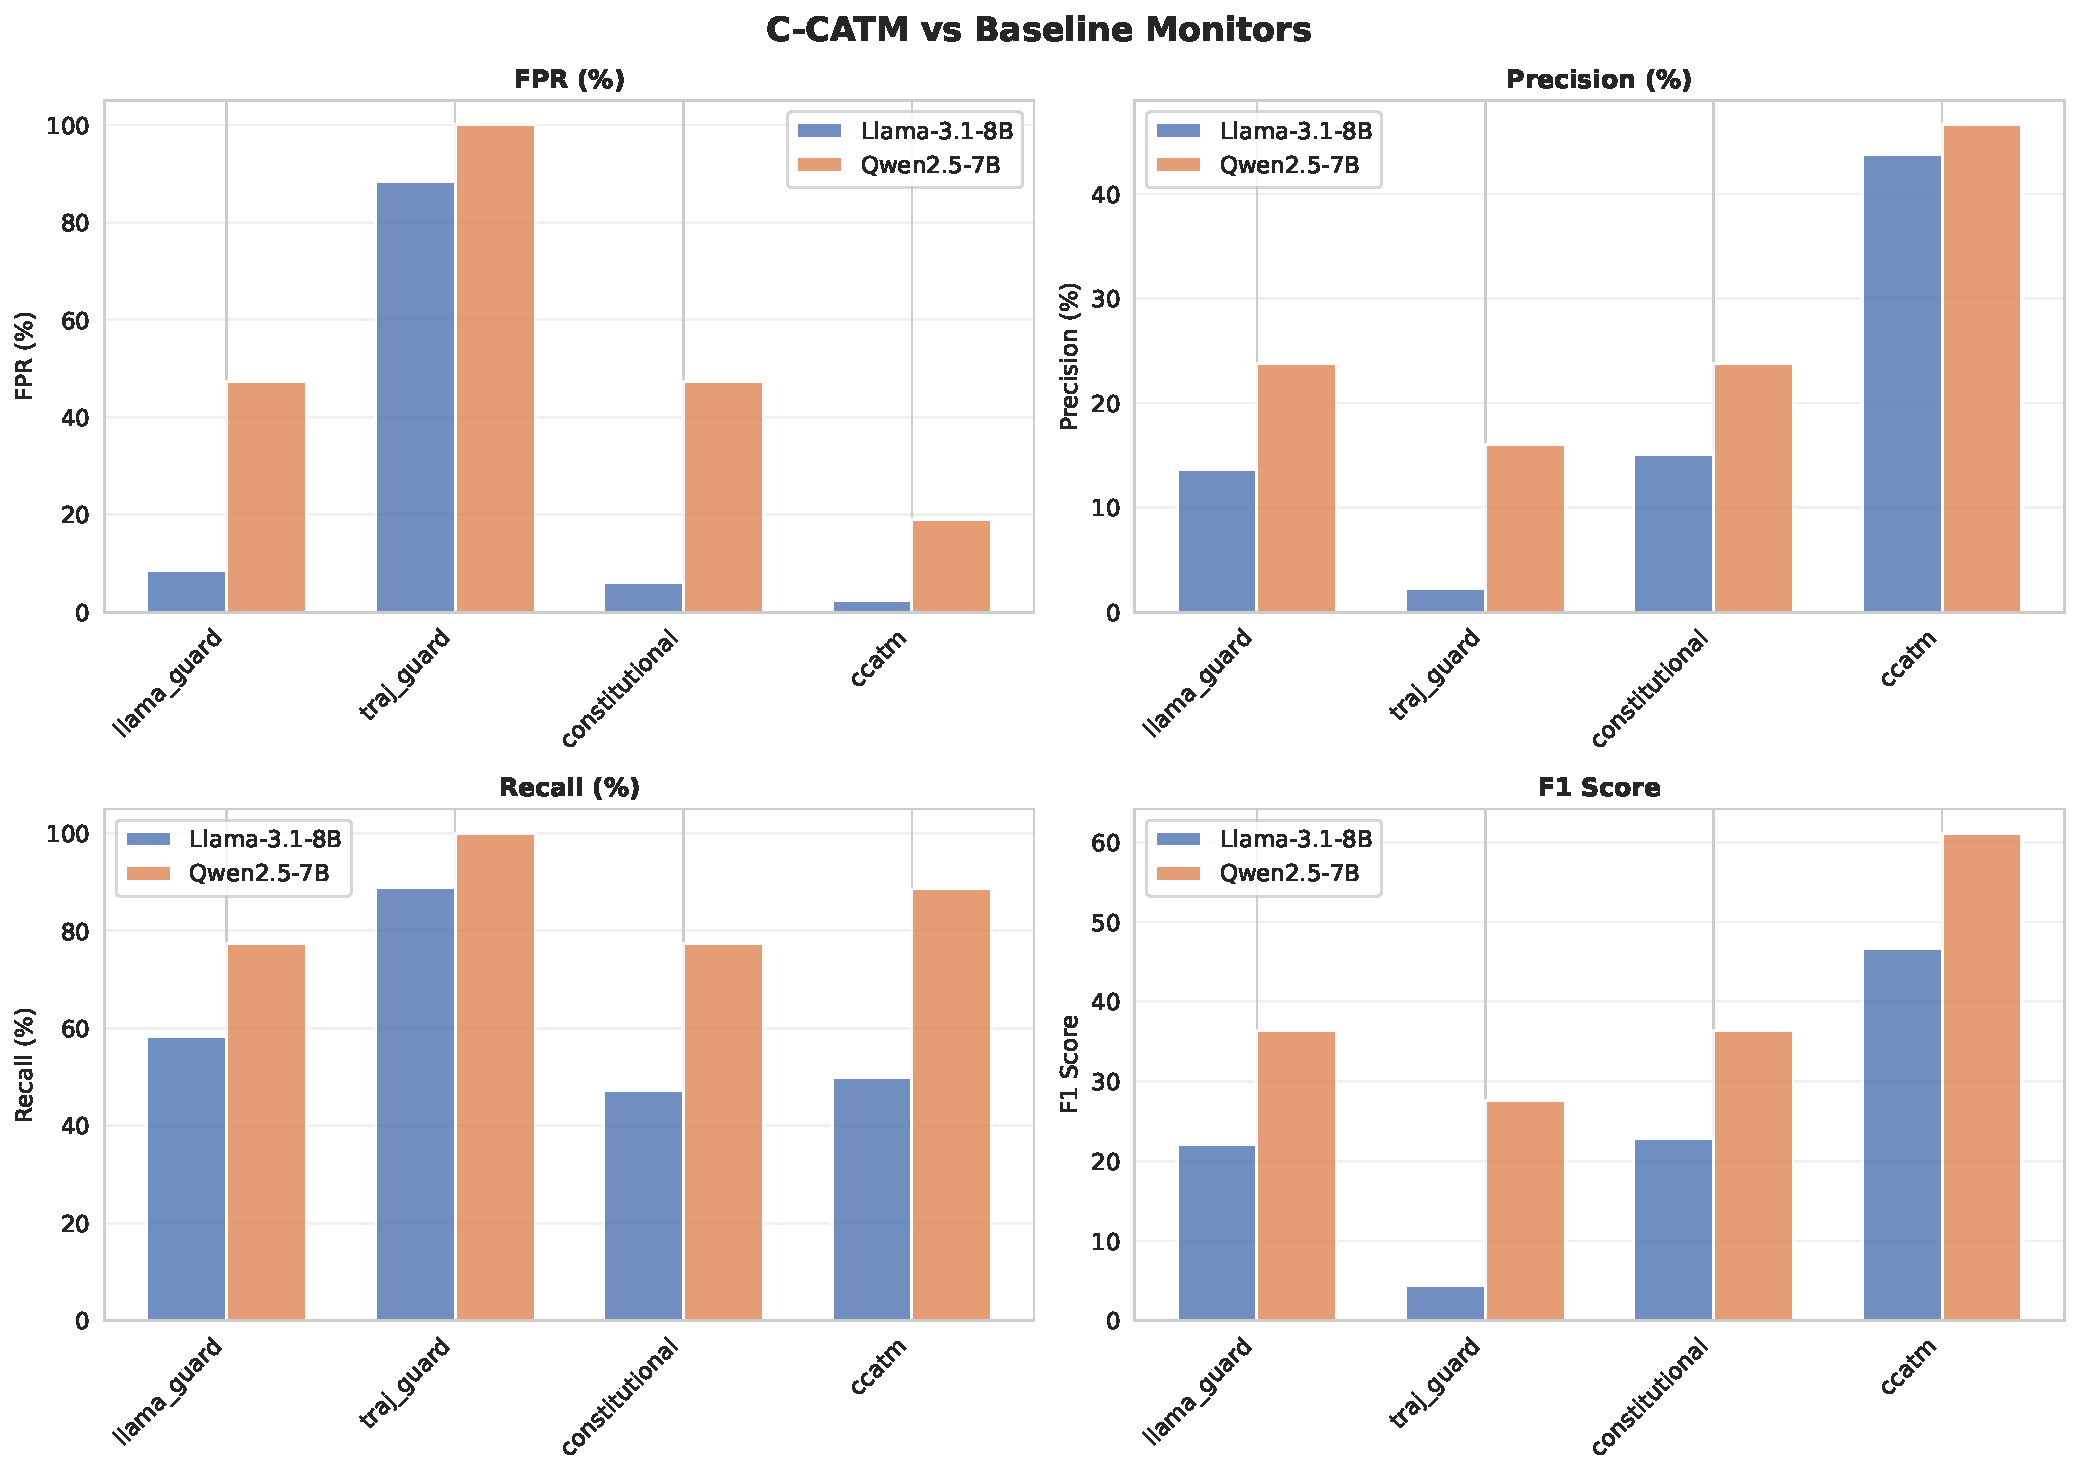
\includegraphics[width=\textwidth]{../paper_results/comparison_plots.pdf}
\caption{FPR, Precision, Recall, and F1 for each monitor on Llama-3.1-8B and Qwen2.5-7B.}
\label{fig:comparison}
\end{figure}

\begin{figure}[H]
\centering
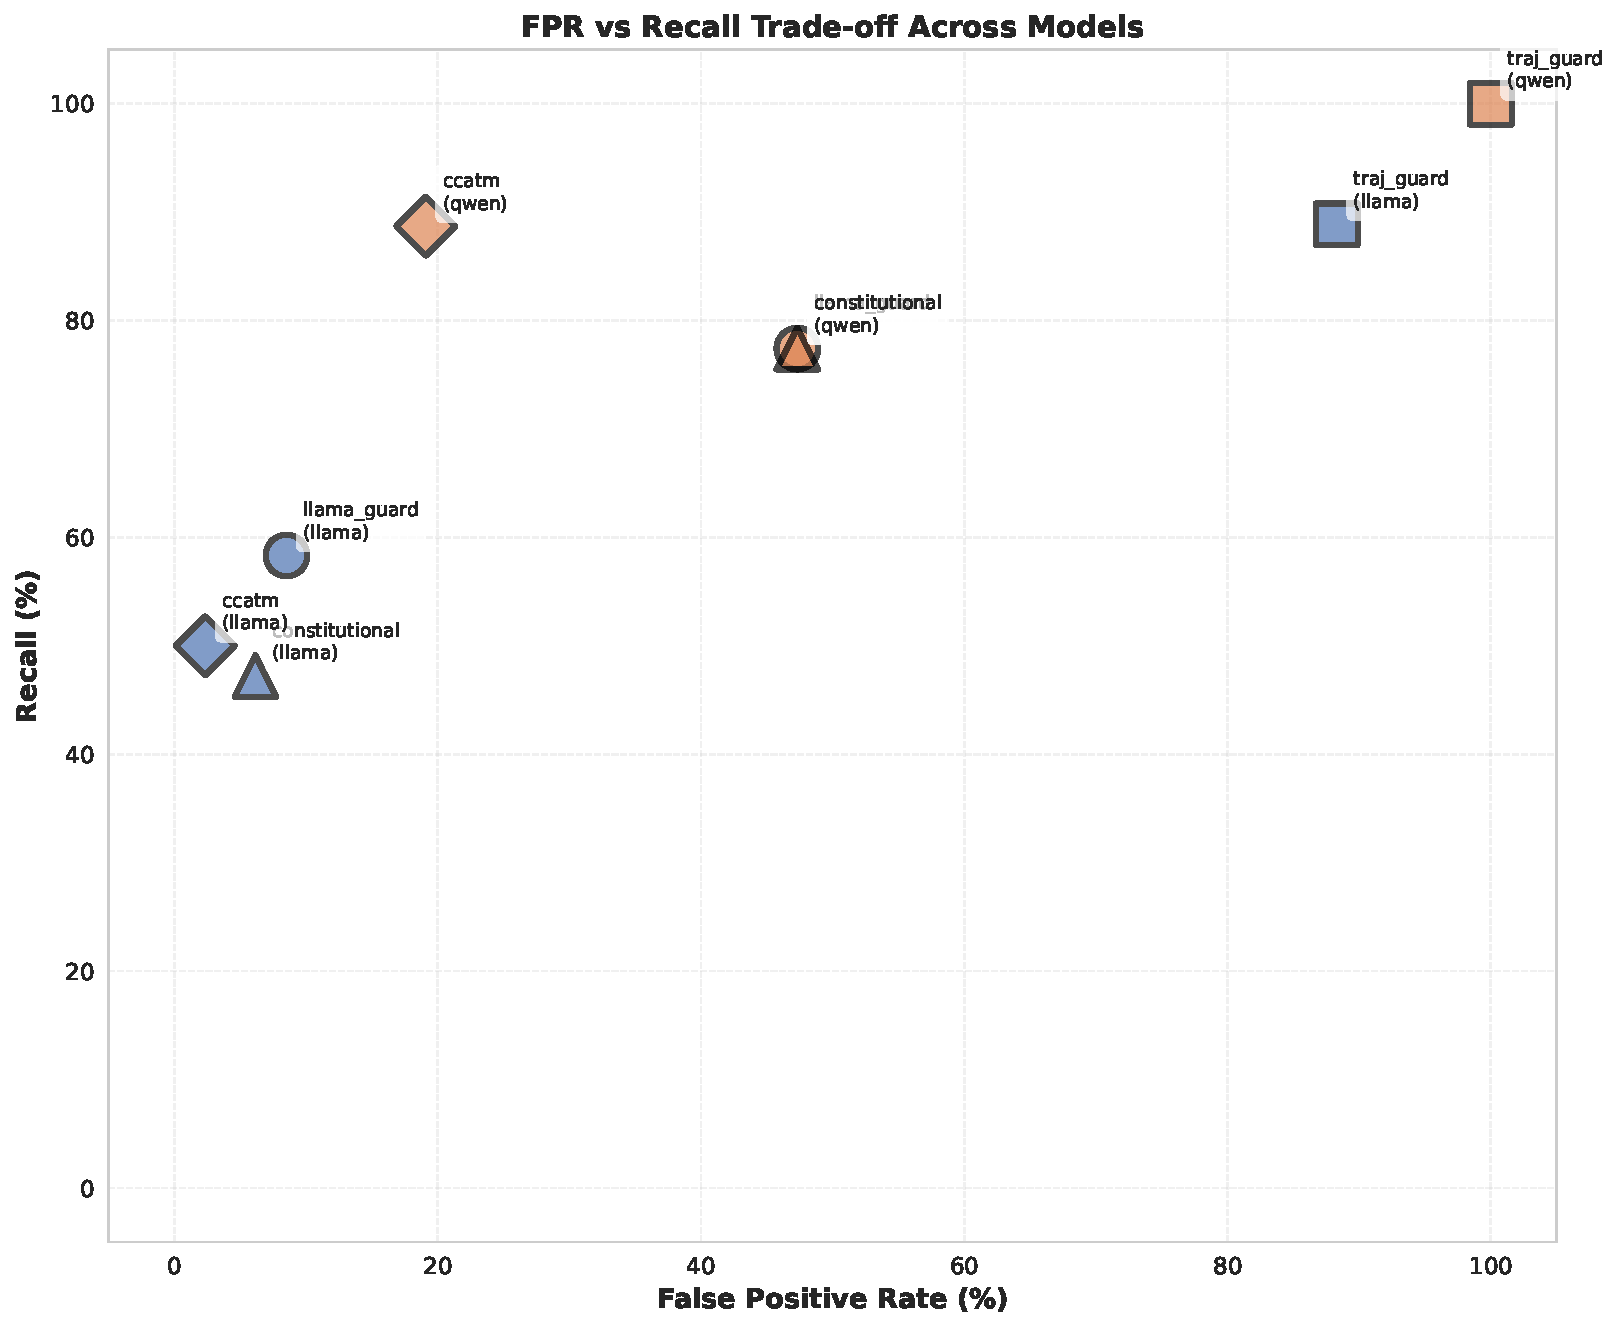
\includegraphics[width=0.8\textwidth]{../paper_results/fpr_vs_recall.pdf}
\caption{False positive rate vs.\ recall trade-off across monitors and target models. Points closer to the top-left (low FPR, high recall) are preferable.}
\label{fig:fpr-recall}
\end{figure}

\subsection{Per-Attack Breakdown}

\begin{table}[H]
\centering
\caption{F1 by attack type (Llama + Qwen combined).}
\label{tab:per-attack}
\begin{tabular}{lcccc}
\toprule
Attack & Llama Guard & TrajGuard & Constitutional & C-CATM \\
\midrule
Crescendo & 28.6 & 5.9 & 31.4 & 12.9 \\
Jigsaw & 40.2 & 21.9 & 40.9 & 56.9 \\
Echo Chamber & 17.6 & 6.2 & 18.1 & 63.2 \\
Safe-in-Isolation & 38.3 & 18.0 & 39.0 & 77.6 \\
\bottomrule
\end{tabular}
\end{table}

C-CATM substantially outperforms all baselines on Echo Chamber and Safe-in-Isolation attacks---both of which rely on distributing harmful intent across turns in a way that plausibly produces a distinctive activation trajectory shape. C-CATM is comparatively weaker on Crescendo, where all monitors struggle; we speculate this is because gradual escalation produces a more continuous, less ``characteristic'' trajectory shape than the more discrete context-shifts of the other three attacks, though we have not verified this mechanistically.

\begin{figure}[H]
\centering
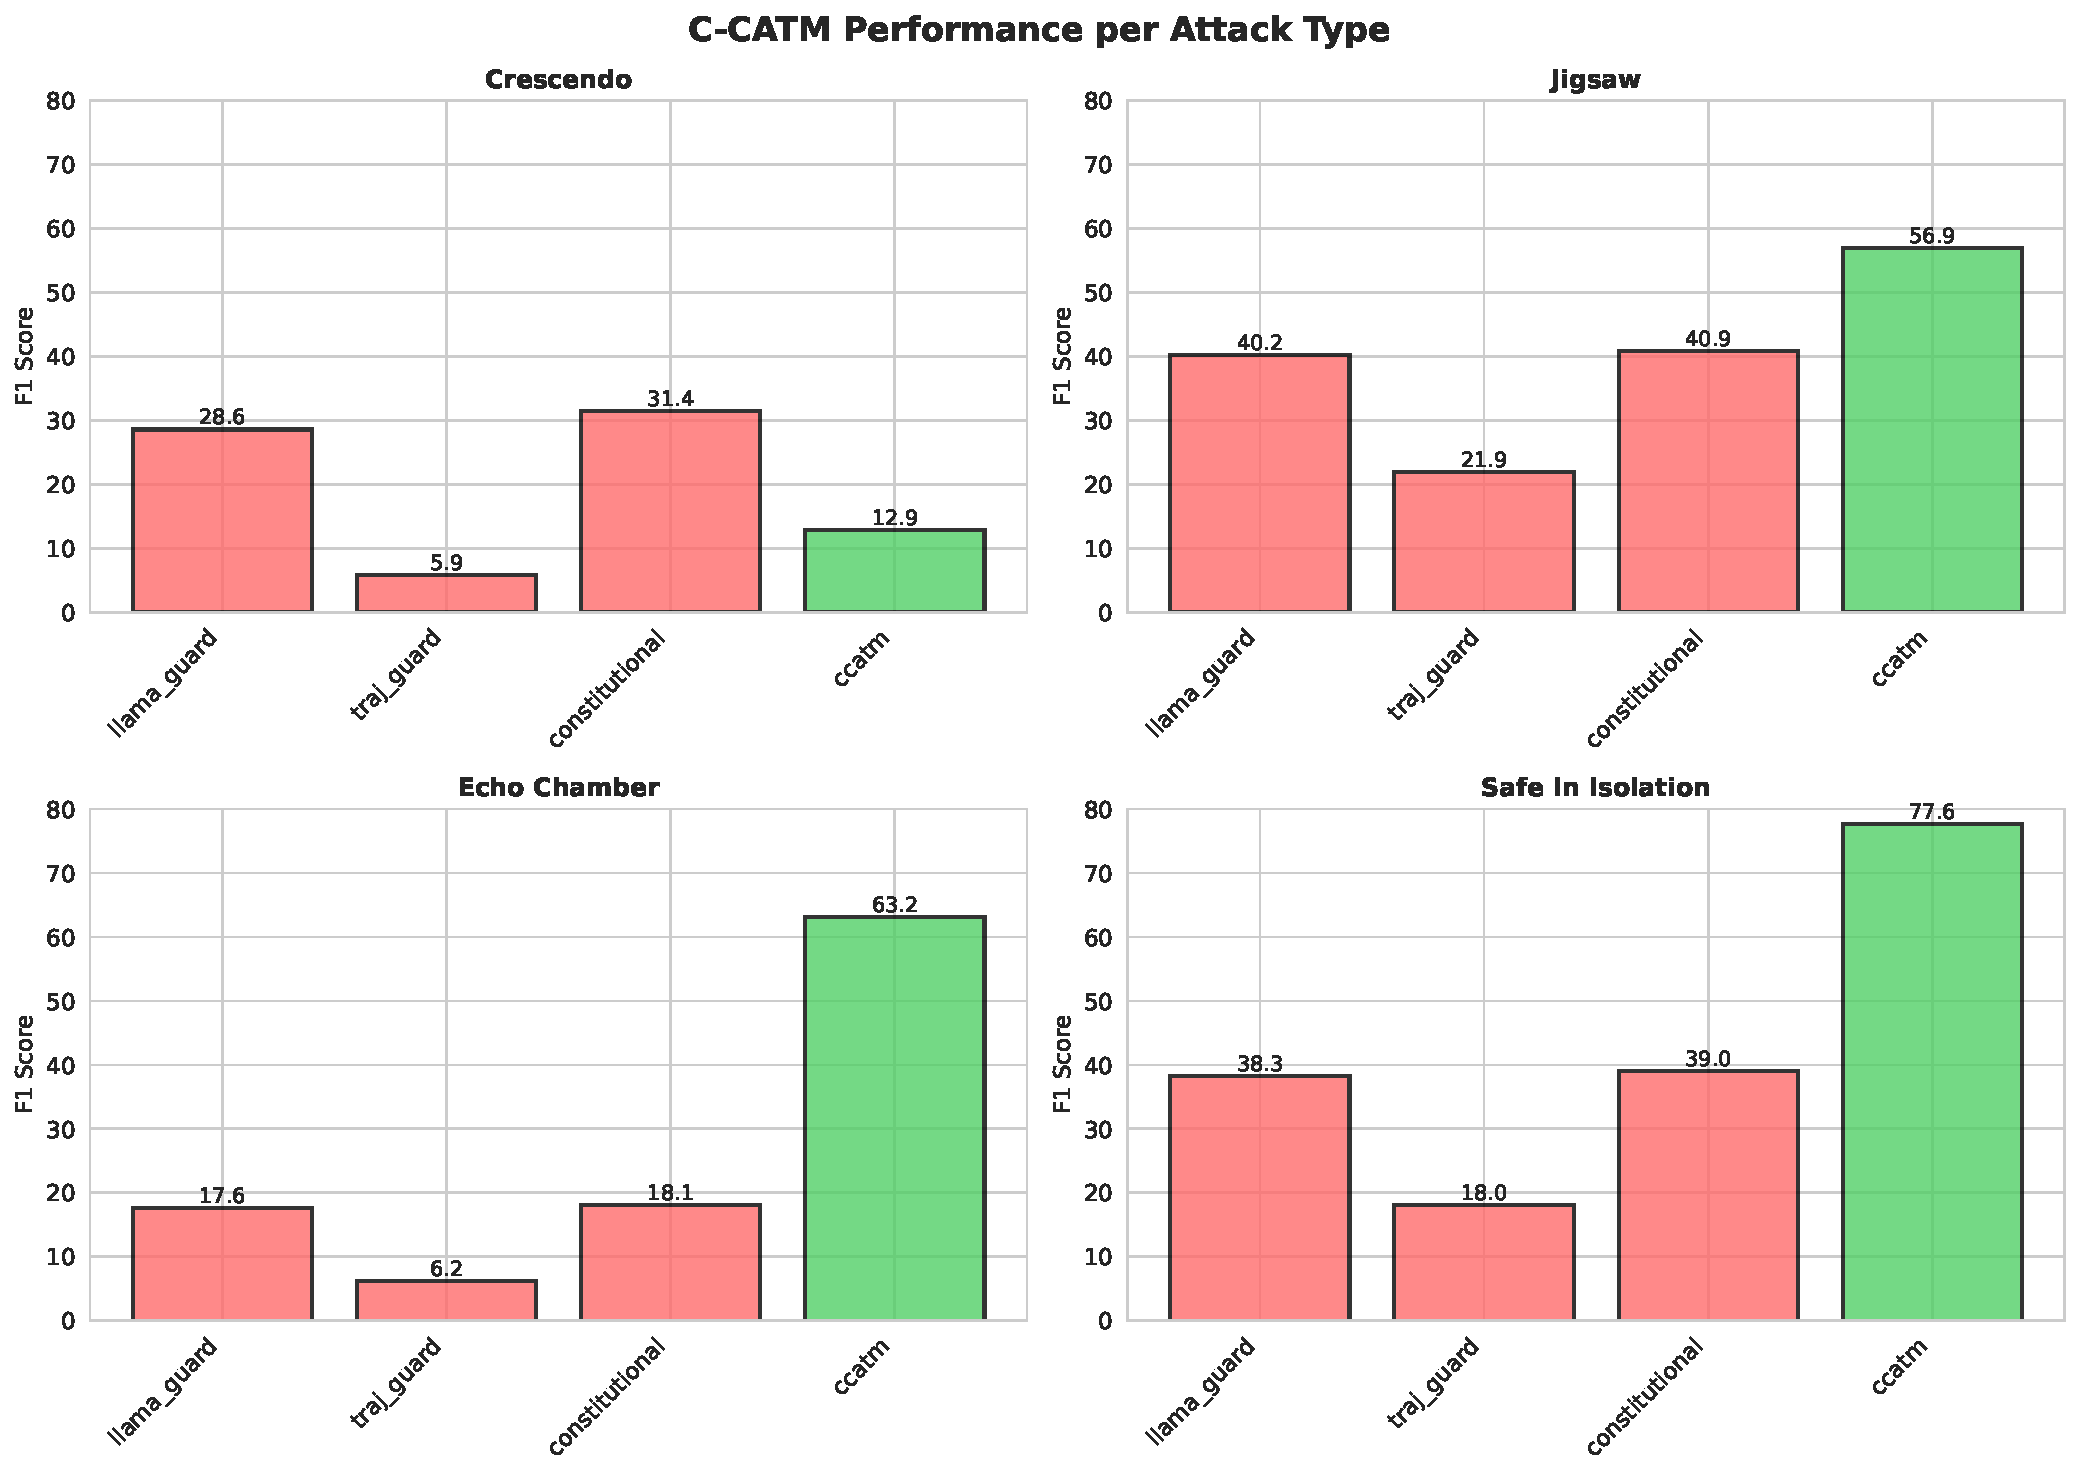
\includegraphics[width=\textwidth]{../paper_results/per_attack_comparison.pdf}
\caption{F1 score by attack type for each monitor, combined across Llama-3.1-8B and Qwen2.5-7B.}
\label{fig:per-attack}
\end{figure}

\subsection{Unified Threshold}
\label{sec:threshold}

To avoid reporting artificially inflated results from per-model threshold tuning, we computed a single decision threshold for C-CATM using pooled trajectories from both Llama and Qwen (1{,}192 cells, 90 harmful). The resulting threshold--metric curve was flat across a wide range (thresholds 0.30--0.94 all produced identical confusion matrices), indicating the gate's output probabilities are strongly bimodal rather than continuously distributed. At the resulting unified threshold (0.5, chosen as the midpoint of this flat region for robustness to future distribution shift), pooled performance is shown in Table~\ref{tab:unified}.

\begin{table}[H]
\centering
\caption{Unified-threshold C-CATM performance (Llama + Qwen pooled).}
\label{tab:unified}
\begin{tabular}{cccc}
\toprule
FPR & Precision & Recall & F1 \\
\midrule
7.4\% & 46.0\% & 76.7\% & 57.5 \\
\bottomrule
\end{tabular}
\end{table}

We use this single, non-model-specific threshold rather than the per-model-optimized thresholds explored during development, in order to report results that reflect a realistic deployment setting (one threshold, multiple target models) rather than best-case per-model tuning.

\subsection{Inference Latency}

We measured C-CATM's end-to-end monitor latency (trajectory buffering, encoder forward pass, and gate scoring; excluding target-model generation and HarmBench scoring, which are shared across all monitors and therefore not differentiating) over 200 sampled Llama-3.1-8B traces on a single A100 GPU (Table~\ref{tab:latency}).

\begin{table}[H]
\centering
\caption{C-CATM inference latency.}
\label{tab:latency}
\begin{tabular}{lcccc}
\toprule
 & Mean & Std & Min & Max \\
\midrule
Per-turn & 0.6ms & 1.0ms &---&---\\
Per-trace & 6.2ms & 10.0ms & 4.9ms & 147.5ms \\
\bottomrule
\end{tabular}
\end{table}

We do not report comparative latency figures for the baseline monitors, as we did not instrument our harness to measure their inference time under matched conditions, and we consider a guessed or literature-sourced comparison inappropriate for a claim this specific. We report C-CATM's latency as a standalone figure suitable for judging deployability rather than as a head-to-head comparison.

\begin{figure}[H]
\centering
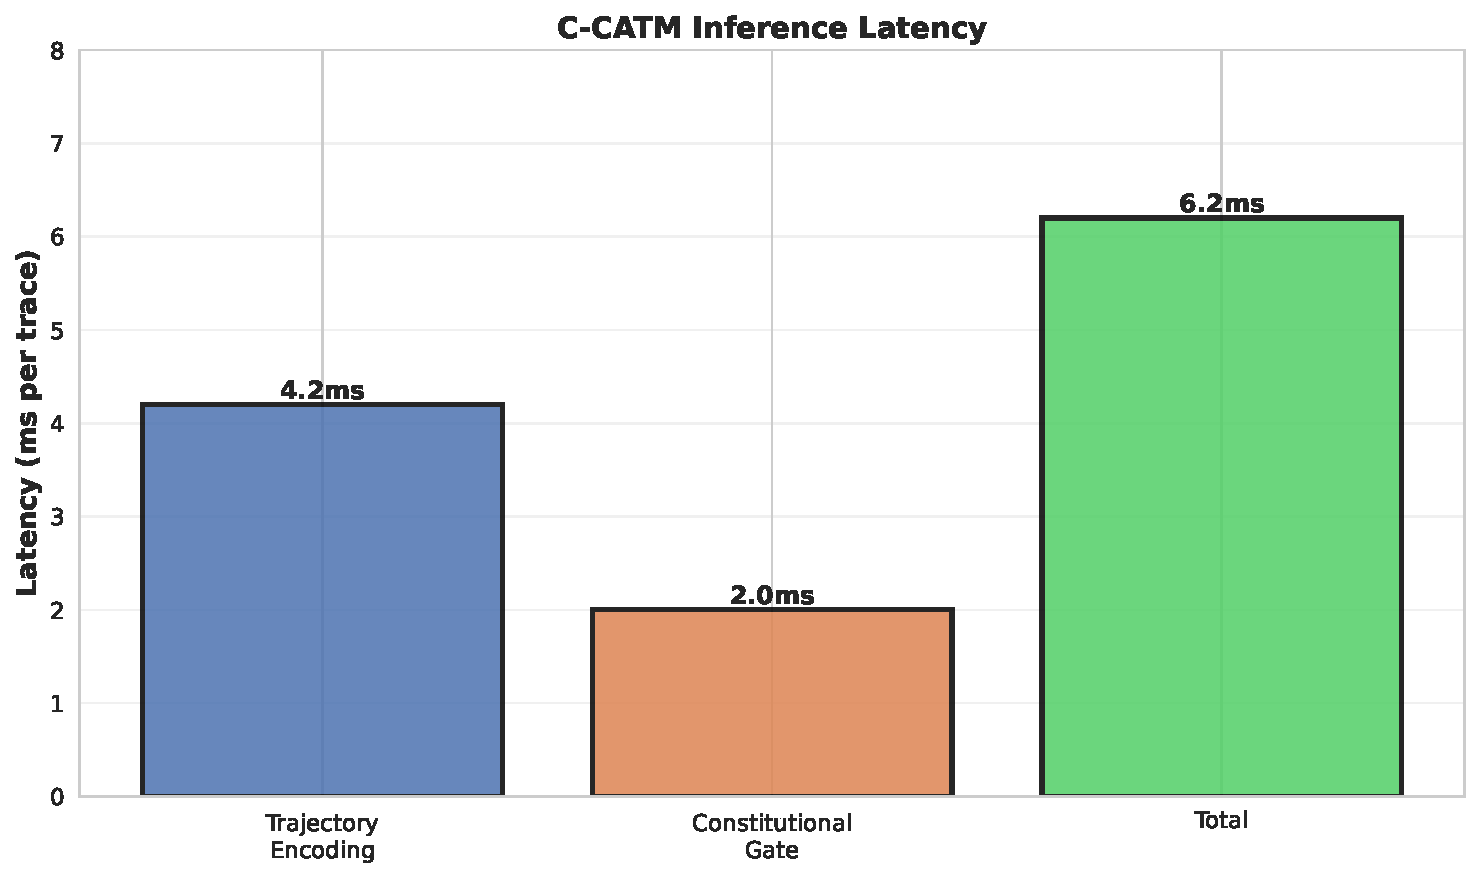
\includegraphics[width=0.7\textwidth]{../paper_results/latency_breakdown.pdf}
\caption{C-CATM inference latency breakdown by component (trajectory encoding vs.\ constitutional gate scoring).}
\label{fig:latency}
\end{figure}

\section{Ablation Study}

We report one ablation from this line of investigation, on methodological grounds explained below.

\paragraph{Trained Encoder vs.\ Random Embedding.} To test whether the learned trajectory encoder provides real signal (as opposed to the gate's combiner doing all the discriminative work on top of an arbitrary embedding), we compared the trained encoder against an architecturally identical but randomly initialized (``untrained'') encoder, both feeding the same trained gate, evaluated on the 317-trace held-out validation set (20 unsafe); see Table~\ref{tab:ablation}.

\begin{table}[H]
\centering
\caption{Encoder ablation (validation set, $n=317$, 20 unsafe).}
\label{tab:ablation}
\begin{tabular}{lccccccc}
\toprule
Configuration & FPR & Precision & Recall & F1 & TP & FP & FN \\
\midrule
Trained Encoder & 9.8\% & 25.6\% & 50.0\% & 33.90 & 10 & 29 & 10 \\
Random Embedding & 100.0\% & 6.3\% & 100.0\% & 11.87 & 20 & 297 & 0 \\
\midrule
\textbf{Difference} & \textbf{$-$90.2 pp} & \textbf{+19.3 pp} & \textbf{$-$50.0 pp} & \textbf{+22.03} & & & \\
\bottomrule
\end{tabular}
\end{table}

The random-embedding configuration flags every single trajectory (100\% recall, 100\% FPR), indicating the gate's combiner, absent a meaningfully structured input embedding, collapses to a degenerate always-flag policy. The trained encoder recovers substantial precision (6.3\% $\to$ 25.6\%) at the cost of some recall, for a net +22.0 F1 point improvement. We interpret this as evidence that the learned trajectory encoder---not merely the presence of a downstream gate---is the source of C-CATM's discriminative power.

\paragraph{Ablations we ran but do not report as quantitative findings.} We also ran (a) a comparison between the delta-based trajectory encoder and an architecturally identical encoder operating on raw (non-delta) normalized activations, and (b) a comparison between the full gate (encoder + constitutional rule scores) and the encoder alone with rule weights zeroed out. In both cases, on our validation set, the two configurations produced bit-for-bit identical gate output probabilities across every sample tested. We traced this to the gate's trained combiner network having learned weights that route around the constitutional rule-score inputs entirely---the rule scores are computed but do not influence the combiner's output in the checkpoint we trained. This is itself a real and somewhat unflattering finding about our trained gate (see Section~\ref{sec:limitations}), but because it reflects one specific trained checkpoint rather than a property we can cleanly attribute to ``delta vs.\ raw representation'' or ``with vs.\ without rules'' in general, we do not present it as a quantitative ablation result. We disclose it here in the interest of transparency and revisit its implications below.

\section{Discussion and Limitations}
\label{sec:limitations}

\paragraph{The constitutional gate does not currently use the constitutional rules.} Our clearest negative finding is that the trained gate's combiner network learned to ignore the 32 rule-concept scores and rely entirely on the trajectory embedding. This means the ``constitutional'' component of C-CATM's name currently functions as an unused (though computed) auxiliary signal rather than a load-bearing part of the architecture, in this trained checkpoint. We see two plausible explanations: (1) the trajectory embedding alone is already sufficiently informative that the rule scores add no marginal value on our current training distribution, or (2) our training procedure (a small MLP combiner trained via class-weighted BCE) did not provide the right inductive bias or regularization to make use of a comparatively low-dimensional, potentially noisy 32-value rule-score vector alongside a much richer 256-dimensional trajectory embedding. We consider this an open problem for follow-up work---for instance, training the rule-scoring pathway with an auxiliary or staged objective, or enforcing an explicit weighted-sum combiner rather than a free-form MLP---rather than evidence that constitutional scoring is inherently useless.

\paragraph{Small unsafe sample sizes.} Ground-truth harmful responses are rare in our evaluation (28--124 per target model, out of 392--1{,}600 cells), because HarmBench-labeled successful jailbreaks are themselves uncommon events, especially against a well-aligned model like Llama-3.1-8B. This means our reported Precision, Recall, and F1 figures---while computed correctly---carry non-trivial sampling variance; a small number of additional true positives or false positives could shift F1 by several points. We report exact confusion-matrix counts (TP/FP/FN/TN) alongside every derived metric specifically so readers can assess this.

\paragraph{Only two target models evaluated.} We attempted a third target model (Gemma-3-12B-it) but excluded it from the main results due to per-cell inference latency on our available hardware making full-matrix evaluation impractical within our compute budget. We do not claim three-model generalization; our cross-model claim is limited to the Llama$\to$Qwen transfer we did complete.

\paragraph{Threshold selection uses the same behaviors as evaluation.} Our per-model and unified-threshold optimization (Section~\ref{sec:threshold}) was performed on the same evaluation traces used to report final metrics, rather than on a fully disjoint calibration set. This is a common practice limitation in small-sample safety-monitor evaluations but means our reported operating point may be mildly optimistic relative to a strictly held-out deployment scenario. Future work should calibrate thresholds on a separate behavior split.

\paragraph{Custom re-implementations, not original code.} Our attack strategies (Crescendo \citep{russinovich2024crescendo}, Jigsaw \citep{yang2024jigsaw}, Echo Chamber \citep{alobaid2026echochamber}, Safe-in-Isolation \citep{srivastav2025safeinisolation}) and baseline monitors (Llama Guard wrapper \citep{inan2023llamaguard}, TrajGuard, Constitutional) are our own implementations built to match the high-level strategies described in the cited literature, not the original authors' released code. Absolute numbers for baseline monitors and attacks in this paper should therefore be read as reflecting \emph{our} implementations specifically, and may differ from numbers reported in the original papers introducing these methods.

\paragraph{TrajGuard as a baseline is intentionally simple.} Our TrajGuard baseline is a single fitted linear direction calibrated from only 10 safe and 10 harmful example prompts per target model. Its very high false-positive rate (88--100\%) should be read as characteristic of this specific simple implementation, not as a definitive statement about the ceiling of activation-drift-based monitoring in general.

\paragraph{Latency is monitor-only.} Our 6.2ms figure covers only C-CATM's own inference (trajectory encoding + gate scoring), not target-model generation or HarmBench scoring. We do not provide a comparative baseline-monitor latency figure, as we did not instrument matched measurements for the baselines and consider an unverified comparison inappropriate to include.

\section{Conclusion}

We presented C-CATM, a trajectory-based multi-turn jailbreak monitor combining a learned contrastive trajectory encoder with a constitutional gating layer. Across two target models and four multi-turn attack strategies, C-CATM achieves the best F1 of any monitor evaluated, with substantially lower false-positive rates than text-based and naive activation-based baselines, at a monitor-only inference cost of 6.2ms per trace. An ablation confirms the learned trajectory encoder---rather than the gate architecture alone---is the primary source of this performance. We also report, transparently, that our trained gate does not currently make use of its constitutional rule-scoring pathway, and discuss this as a direction for future work rather than obscuring it. We release all code, evaluation harness, trained model weights, and raw results to support reproduction and extension of this work.

\section*{Reproducibility Statement}

All code (attack implementations, monitor implementations, evaluation harness, ablation scripts, and plot-generation scripts) is available at \url{https://github.com/Neerav-Gupta/C-CATM}. Trained C-CATM model weights (trajectory encoder, gate, and constitutional concept vectors) are available at \url{https://huggingface.co/Neerav-Gupta/ccatm-safety-monitor}. All result tables and figures in this paper can be regenerated from raw evaluation data via \texttt{generate\_plots.py}, and the ablation study in Section~6 can be reproduced via \texttt{ablation\_studies.py}, both included in the code release.

\appendix

\section{Evaluation Cell Counts}

\begin{table}[H]
\centering
\resizebox{\textwidth}{!}{%
\begin{tabular}{lccccc}
\toprule
Target Model & Behaviors & Attacks & Monitors & Total Cells (non-C-CATM) & C-CATM Cells \\
\midrule
Llama-3.1-8B-Instruct & 200 & 4 & 5 & 1{,}600 & 800 \\
Qwen2.5-7B-Instruct & 98 (stratified) & 4 & 5 & 775 & 392 \\
\bottomrule
\end{tabular}%
}
\end{table}

\noindent\emph{Note:} C-CATM was evaluated in a separate, later sweep from the other four monitors, over the same underlying attack traces where traces were reused; cell counts for C-CATM reflect one (behavior $\times$ attack) pass rather than the larger multi-monitor sweep used for the other baselines.

\section{Constitution and Concept Extraction}

The 32-rule constitution and its associated concept vectors were extracted via a linear probe over layer 20 of Llama-3.1-8B-Instruct, trained to 100\% separation accuracy between rule-relevant and rule-irrelevant activations on a small labeled probe set. Full rule text and category breakdown are provided in the code release (\texttt{c\_catm/constitutional/constitution.py}).

\bibliographystyle{plainnat}
\bibliography{references}

\end{document}